\documentclass[serif,xcolor=pdftex,dvipsnames,table,hyperref={bookmarks=false,breaklinks}]{beamer}

%%%%%%%%%%%%%%%%
% Change the macros below to configure the title slides
% for your course.
\newcommand{\coursename}{COMPSCI 589}
\newcommand{\instructor}{Benjamin M. Marlin}
\newcommand{\university}{University of Massachusetts Amherst}
\newcommand{\department}{College of Information and Computer Sciences}
%%%%%%%%%%%%%%%%


\newcommand{\settitlecard}[2]{
  \title[\coursename  Lecture #1] 
    {\coursename \\ Lecture #1: #2}
     \author[\instructor]{\instructor}
     \institute[\university]{
     \department\\
     \university
   }
\date{}
}

\newcommand{\maketitlepage}{
  \begin{frame}
  \titlepage
  \center{
    %If you use the slides unmodified, retain the attribution below
    \tiny{Slides by Benjamin M. Marlin (marlin@cs.umass.edu). \\
    \vspace{-1em}Created with support from National Science Foundation Award\# IIS-1350522. 
    %If you modify the slides, please retain the alternate attribution below
    %\tiny{Based on slides by Benjamin M. Marlin (marlin@cs.umass.edu). \\    
    %\vspace{-1em}Created with support from National Science Foundation Award\# IIS-1350522. 
    }                                              
  }  
  \end{frame}
}

\AtBeginSection[]
{
  \begin{frame}<beamer>{Outline}
    \tableofcontents[currentsection,subsectionstyle=hide]
  \end{frame}
}


\newcommand{\cut}[1]{}

\newcommand{\iconbox}[4]{
  \only<#1-#2>{
    \begin{columns}[T]
      \column{0.5in}
           \includegraphics[width=0.5in]{#3}
       \column{3.7in}
            #4
    \end{columns}
    \medskip
    \medskip
    \medskip
  }
}

\mode<presentation>{
  \usepackage{../beamertheme589theme}
  \setbeamercovered{invisible}
}

\mode<handout>{
  \usepackage{../beamertheme589theme}
  \setbeamercovered{transparent}
}


\usepackage[english]{babel}
\usepackage[latin1]{inputenc}
\usepackage{times}
\usepackage[T1]{fontenc}
\usepackage{amsmath}
\usepackage{amssymb}
\usepackage[noend]{algorithmic}
\usepackage{algorithm}
\usepackage{listings}

\renewcommand\mathfamilydefault{\rmdefault}

\newcommand{\setA}{\mathcal{A}}
\newcommand{\setB}{\mathcal{B}}
\newcommand{\setS}{\mathcal{S}}
\newcommand{\setV}{\mathcal{V}}
\DeclareMathOperator*{\union}{\bigcup}
\DeclareMathOperator*{\intersection}{\bigcap}
\DeclareMathOperator*{\Val}{Val}
\newcommand{\mbf}[1]{{\mathbf{#1}}}
\DeclareMathOperator*{\argmax}{arg\,max}
\DeclareMathOperator*{\argmin}{arg\,min}
\DeclareMathOperator*{\sign}{sign}
\newcommand{\deriv}[2]{\frac{\partial{#1}}{\partial{#2}}}


\settitlecard{9}{KNN Regression, Regression Trees, \\and Feature Selection}

\begin{document}

\maketitlepage

\section{Review}
\subsection{Foo}

\begin{frame}[t]{The Regression Task}

\begin{block}{Definition: The Regression Task}
Given a feature vector $\mbf{x}\in\mathbb{R}^D$, predict it's corresponding output value $y$.
\end{block}

\center
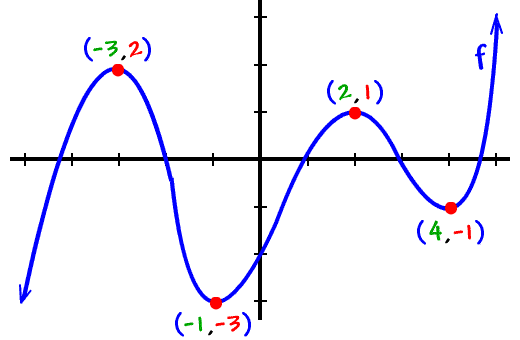
\includegraphics[width=3in]{../Figures/polynomial-function.png}
\end{frame}

\begin{frame}[t]{The Regression Learning Problem}
\begin{block}{Definition: Regression Learning Problem}
Given a data set of example pairs $\mathcal{D}=\{(\mbf{x}_i,y_i),i=1:N\}$ where $\mbf{x}_i\in\mathbb{R}^D$ is a feature vector and $y_i\in \mathbb{R}$ is the output, learn a function $f:\mathbb{R}^D\rightarrow \mathbb{R}$ that accurately predicts $y$ for any feature vector $\mbf{x}$.
\end{block}
\end{frame}

\begin{frame}[t]{Error Measures: MSE}
\begin{block}{Definition: Mean Squared Error}
Given a data set of example pairs $\mathcal{D}=\{(\mbf{x}_i,y_i),i=1:N\}$ and a function $f:\mathbb{R}^D\rightarrow \mathcal{Y}$, the mean squared error of $f$ on $\mathcal{D}$ is:
$$MSE(f,\mathcal{D}) = \frac{1}{N}\sum_{i=1}^N(y_i - f(\mbf{x}_i))^2$$
\end{block}
\pause

Related measures include: \\
Sum of Squared Errors: $SSE(f,\mathcal{D})=N\cdot MSE(f,\mathcal{D})$\\
Risidual Sum of Squares: $RSS(f,\mathcal{D})=N\cdot MSE(f,\mathcal{D})$\\
Root Mean Squared Error: $RMSE(f,\mathcal{D})=\sqrt{MSE(f,\mathcal{D})}$


\end{frame}

\section{KNN Regression}
\subsection{foo}

\begin{frame}[t]{K Nearest Neighbors Regression}

The KNN regression is a non-parametric regression method that simply stores the training data $\mathcal{D}$
and makes a prediction for each new instance $\mbf{x}$ using an average over it's set of $K$ nearest neighbors $\mathcal{N}_K(\mbf{x})$ computed using any distance function $d:\mathbb{R}^D \times\mathbb{R}^D \rightarrow \mathbb{R} $.

\pause
\begin{block}{KNN Regression Function}
$$f_{KNN}(\mbf{x}) = \frac{1}{K}\sum_{i\in \mathcal{N}_K(\mbf{x})} y_i$$
\end{block}

\pause As with classification, use of KNN requires choosing the distance function $d$ and the number of neighbors $K$.
\end{frame}



\begin{frame}[t]{Example: 1D KNN (K=1 vs K=9)}

\center
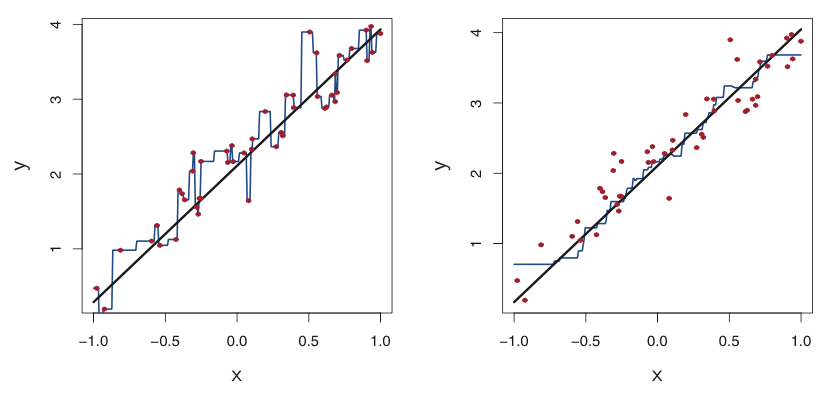
\includegraphics[width=4in]{../Figures/knn_regression_1d.png}

\end{frame}

\begin{frame}[t]{Example: 2D KNN (K=1 vs K=9)}

\center
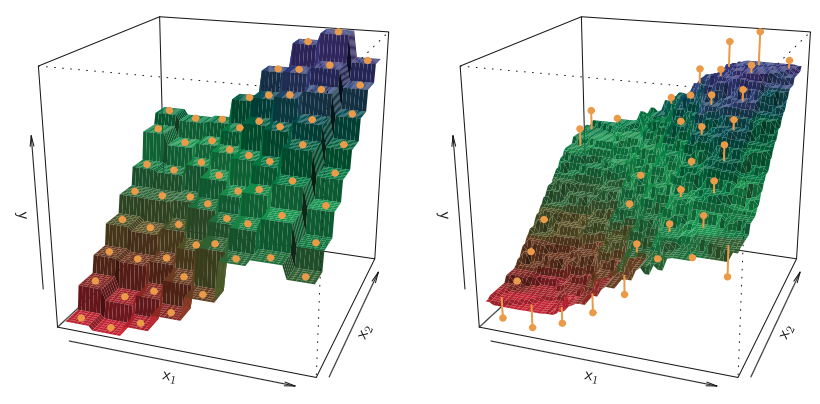
\includegraphics[width=4in]{../Figures/knn_regression_2d.png}

\end{frame}


\begin{frame}[t]{Weighted KNN Regression}

\begin{itemize}
\item Instead of giving all of the $K$ neighbors equal weight in the average, a distance-weighted average can be used:

\begin{align*}
f_{KNN}(\mbf{x}) &=\frac{\sum_{i\in \mathcal{N}_K(\mbf{x})} w_i y_i}
{\sum_{i\in \mathcal{N}_K(\mbf{x})} w_i}\\
w_i &= \exp(-\alpha d_i)
\end{align*}

\end{itemize}

\end{frame}


\section{Regression Trees}
\subsection{Foo}

\begin{frame}[t]{Regression Trees}
\center
\begin{itemize}
\item A regression tree makes predictions using a conjunction of rules organized into a binary tree structure.

\pause\item Each internal node in a regression tree contains a rule of the form $(x_d<t)$ or $(x_d=t$) that tests a single data dimension $d$ against a single threshold value $t$ and assigns the data case to it's left or right sub-tree according to the result.

\pause \item A data case is routed through the tree from the root to a leaf. Each leaf node is associated with a predicted output, and a data case is assigned the output of the leaf node it is routed to.

\end{itemize}

\end{frame}

\begin{frame}[t]{Example: 2D Regression Trees}
\center
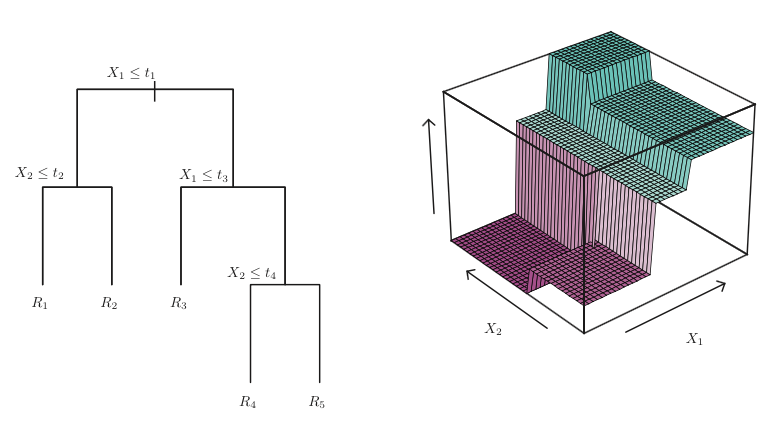
\includegraphics[page=1,width=4in]{../Figures/2DTree-Example.png}
\end{frame}

\begin{frame}[t]{Building Regression Trees}
\center
\begin{algorithm}[H]
\caption{$BuildTree(Root,\mathcal{D},h,minS,maxD)$}
\begin{algorithmic}
\STATE  $d,t = BestSplit(\mathcal{D})$
\pause\STATE  $\mathcal{D}_1 = \{(y_i,\mbf{x}_i)| x_{di}\leq t\}$, $\mathcal{D}_2 = \{(y_i,\mbf{x}_i)| x_{di} > t\}$
%
\pause\IF{$|\mathcal{D}_1|<=minS$ or $h+1\geq maxD$}
\pause  \STATE  $Root.RightChild.Prediction = \frac{1}{|\mathcal{D}_1|}\sum_{y \in \mathcal{D}_1} y$
\pause\ELSE 
\pause \STATE $BuildTree(Root.RightChild, \mathcal{D}_1,h+1,minS,maxD)$
\pause\ENDIF   
%     
\pause\IF{ $|\mathcal{D}_2|<=minS$ or $h+1\geq maxD$}
\pause  \STATE  $Root.LeftChild.Prediction = \frac{1}{|\mathcal{D}_2|}\sum_{y \in \mathcal{D}_2} y$
\pause\ELSE
\pause  \STATE $BuildTree(Root.LeftChild, \mathcal{D}_2,h+1,minS,maxD)$
\pause\ENDIF 
\pause  \STATE $Root.d=d$,$Root.t=t$
\pause\RETURN{$Root$} 
\end{algorithmic}
\end{algorithm}
\end{frame}



\begin{frame}[t]{Finding the Best Split}
\center
\begin{algorithm}[H]
\caption{$BestSplit(\mathcal{D})$}
\begin{algorithmic}
\pause\FOR{$d$ from $1$ to $D$}
\pause  \STATE $\mathbf{s} = sort(\{x_{d1},...,x_{dN}\})$
\pause  \FOR{$t$ in $\{(s_i+s_{i+1})/2|i=1...N-1\}$}
\pause    \STATE $\mathcal{D}_1 = \{(y_i,\mbf{x}_i)| x_{di}\leq t\}$
\pause    \STATE $\mathcal{D}_2 = \{(y_i,\mbf{x}_i)| x_{di} > t\}$
\pause    \STATE $\bar{y}_1 = \frac{1}{|\mathcal{D}_1|}\sum_{y \in \mathcal{D}_1} y$
\pause    \STATE $\bar{y}_2 = \frac{1}{|\mathcal{D}_2|}\sum_{y \in \mathcal{D}_2} y$
\pause    \STATE $Score(d,t) = \sum_{y \in \mathcal{D}_1} (y-\bar{y}_1)^2 + \sum_{y \in \mathcal{D}_2} (y-\bar{y}_2)^2$
\pause  \ENDFOR
\pause\ENDFOR
\pause\STATE $d,t = \argmin_{d',t'}  Score(d,t)$
\pause\RETURN{ $(d,t)$}
\end{algorithmic}
\end{algorithm}
\end{frame}

\begin{frame}[t]{Example: Building Regression Trees}
\center
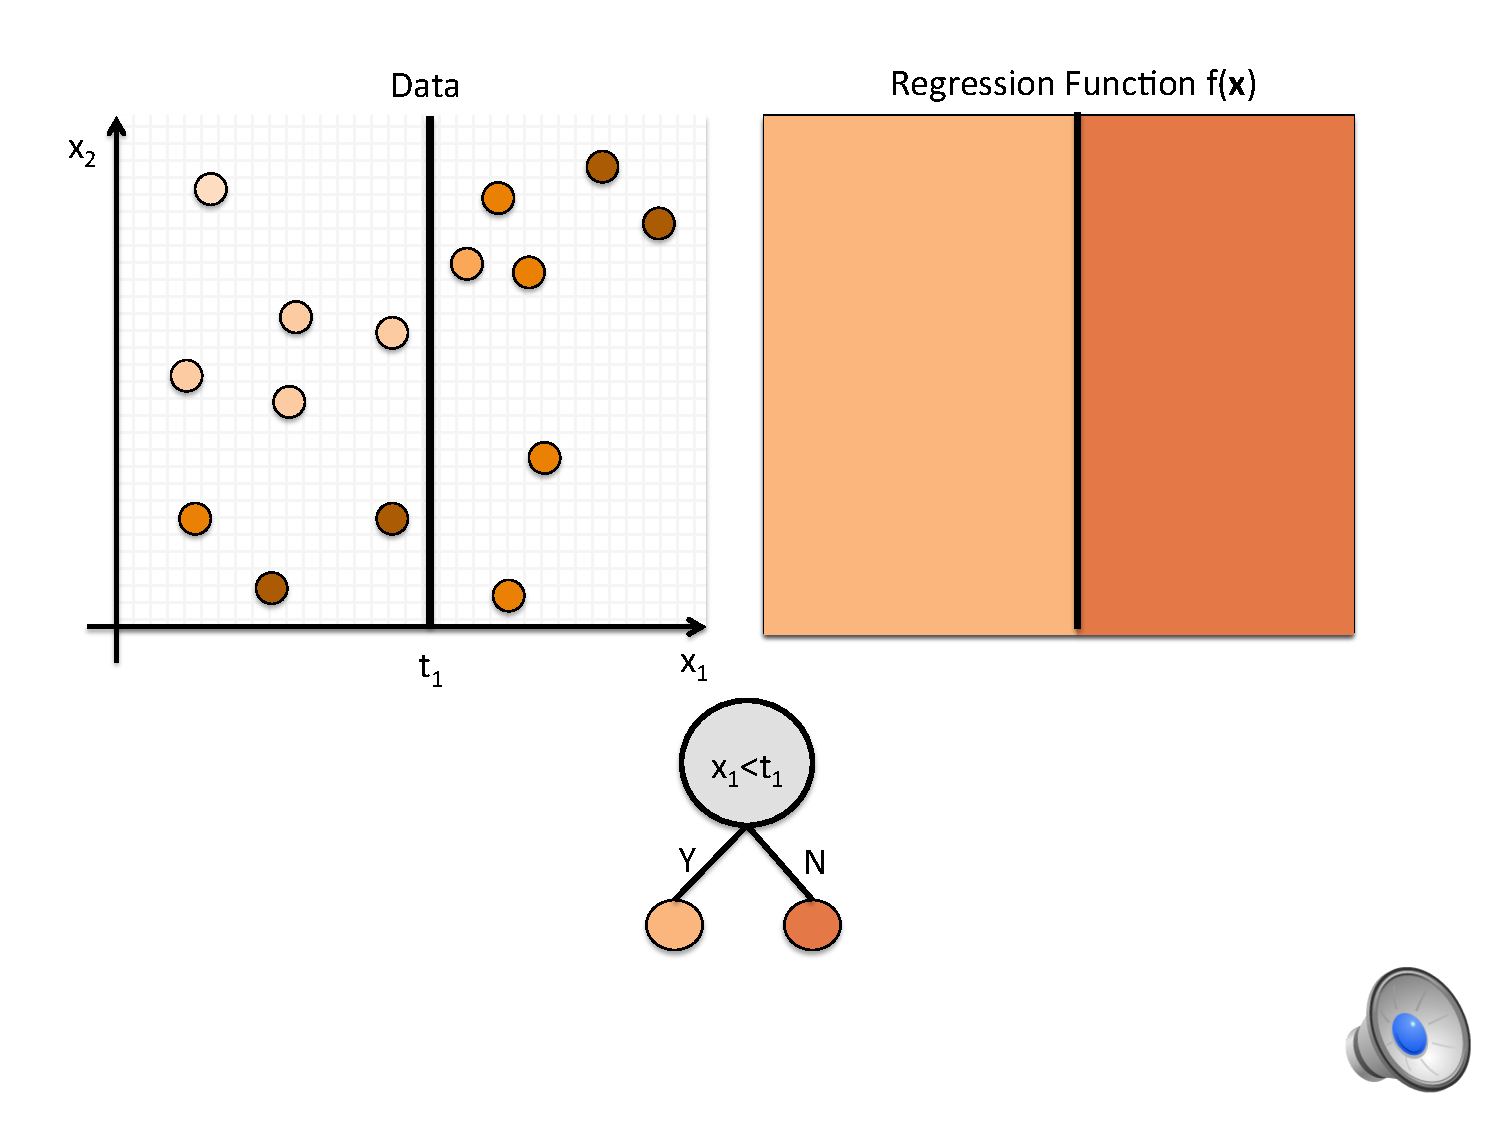
\includegraphics[page=1,width=3.5in]{../Figures/regression_tree.pdf}
\end{frame}

\section{Feature Selection}
\subsection{foo}

\begin{frame}[t]{Best Subset Selection}
\center
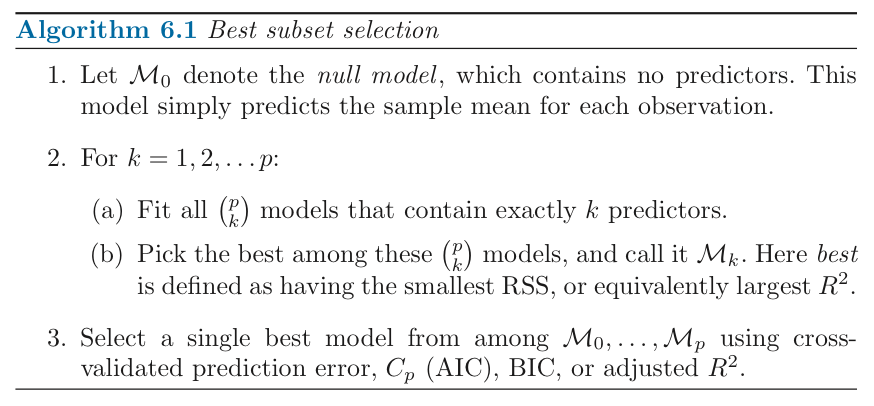
\includegraphics[width=4in]{../Figures/best_subset_selection.png}

\end{frame}

\begin{frame}[t]{Forward Stepwise Selection}
\center
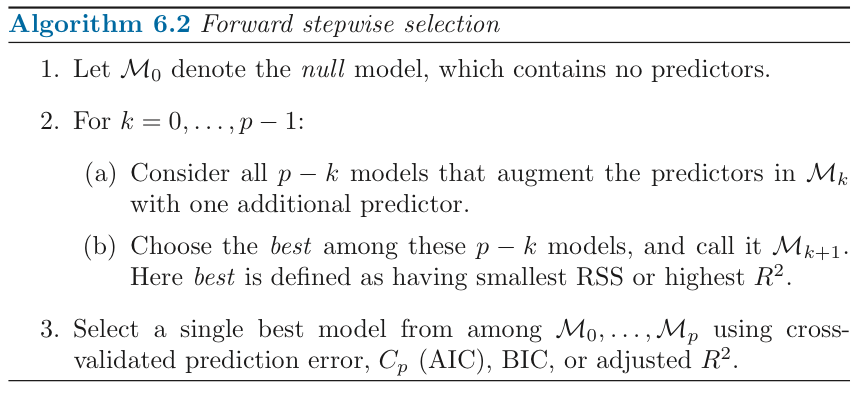
\includegraphics[width=4in]{../Figures/forward_selection.png}
\end{frame}

\begin{frame}[t]{Backward Stepwise Selection}
\center
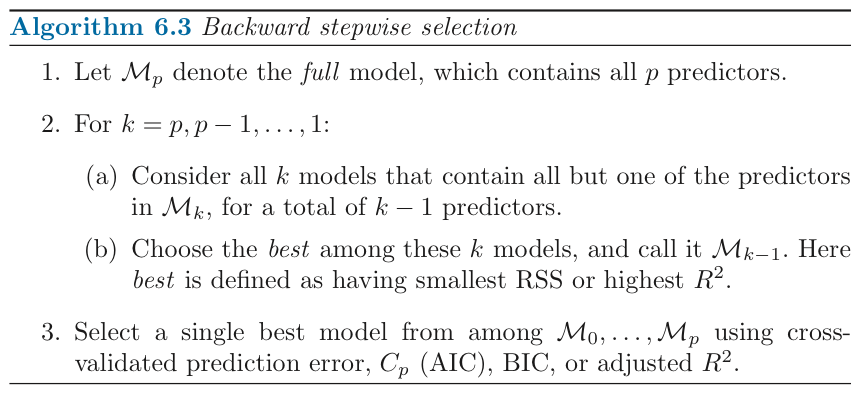
\includegraphics[width=4in]{../Figures/backward_selection.png}
\end{frame}




\end{document}
